\subsection{Synthetic Data}

First, tests were run on data generated in situ from a list of frequencies,
coefficients, and phase differences

\begin{align*}
    c &= \{c_1, c_2, \ldots, c_n\}\\
    \omega &= \{\omega_1, \omega_2, \ldots, \omega_n\}\\
    \phi &= \{\phi_1, \phi_2, \ldots, \phi_n\}\\
\end{align*}

which generate a 'generating' function for the discrete signal to follow

\begin{align*}
    f(x) = \sum_{i = 1}^{n} c_i \cdot sin(w_i x + \phi_i)
\end{align*}

implemented as a lambda-function in code 

\begin{lstlisting}[language=C++]
auto f_gen = [w, c, p](int x){
                float sum = 0;
                for(int i = 0; i < wlist.size(); i++){
                    sum += c[i] * sin(w[i]*x + p[i]);
                }
                return 7.0*sum/float(std::accumulate(c.begin(), c.end(), 0));
            };
            
auto f = new signal[SIZE];

for(int x = 0; x < SIZE; x++){
    f[i] = signal(f_gen(2*x), f_gen(2*x + 1));
}
\end{lstlisting}

The normalising factor may be succinctly written as 

\begin{align*}
    a_N = \frac{7.0}{\sum_{i = 1}^{n}c_i}~.
\end{align*}

It simply ensures that the cross correlation of the signals do not blow up and
that a single signal agnostic threshold value may be chosen as a metric for
matching. The factor of 7 scales the float value to the range (-7, 7) so as to
maintain reasonable resolution after conversion to integer type to save memory.

The signal is generated as even/odd pairs to facilitate pairwise storage
implemented by \nameref{sec:doobit}. The typename \texttt{signal} is an alias
for \texttt{doobit}, kept as such for modularity amongst storage backends, and
to possibly expand across architectures, saving major edits.

Playing with the described parameters, experiments were performed, and the
results have been tabulated in \autoref{fig:synthexp}. Since we look for a
global maxima of cross correlation, the phase is irrelevant to the results, but
for the sake of completeness, an indication has been provided where phase shifts
were tested. Several arbitrary values were tested, with the result being
uneaffected as expected.

All synthetic tests were performed with a resolution of 1ms, and 400 data points.

\begin{figure}[ht]
    \centering
    \def\arraystretch{1.5}
    \setlength\tabcolsep{2em}
    \begin{tabular}{c | c | c}
        NCC Threshold (t)   & Input frequencies and coefficients (kHz)      & Output (kHz)  \\ \hline
        0.1                 & 0.3, 0.5, 0.8                                 & 0.3, 0.5, 0.8 \\
        0.1                 & 0.3, 0.5, 0.8$^\dagger$                       & 0.3, 0.5, 0.8 \\
        0.1                 & 0.3, 0.5$^\dagger$, 0.8$^\dagger$             & 0.3, 0.5, 0.8 \\
        0.2                 & 0.3, 0.5$^\dagger$, 0.8$^\dagger$             & 0.3, 0.5, 0.8 \\
        0.2                 & 0.3, 0.5$^\dagger$, 0.8$^\dagger$             & 0.3, 0.5, 0.8 \\
        0.2                 & 0.3, 4$\times$ 0.5$^\dagger$, 0.8$^\dagger$   & 0.3, 0.5, 0.8 \\
        0.4                 & 0.3, 4$\times$ 0.5$^\dagger$, 0.8$^\dagger$   & 0.3, 0.5, 0.8 \\
        0.5                 & 0.3, 4$\times$ 0.5$^\dagger$, 0.8$^\dagger$   & 0.3, 0.5      \\
        0.6                 & 0.3, 4$\times$ 0.5$^\dagger$, 0.8$^\dagger$   & 0.5           \\
        0.8                 & 0.3, 4$\times$ 0.5$^\dagger$, 0.8$^\dagger$   & $\emptyset$   \\
        0.1                 & 0.3, 0.5, 0.35$^\dagger$                      & 0.3, 0.4, 0.5 \\
        0.2                 & 0.3, 0.5, 0.35$^\dagger$                      & 0.3, 0.5     
    \end{tabular}
    \captionsetup{justification=centering}
    \caption{Experiments with varying synthetic inputs and thresholds.\\
    $\dagger.$ Phase shifted. Weight unit unless otherwise specified}
    \label{fig:synthexp}

\end{figure}

\subsection{Real Inputs}

Not having a microphone module for the Arduino, we resorted to passing a
recorded array to the device via MATLAB, opening its own can of worms by way of
buffer overflows and race conditions, as described in detail in
\autoref{subsec:buffinp}. 

For currently unknown reasons, we had memory overflows with the same size of
real data as we ran synthetic tests for. Curiously, in this case, the Arduino
continuosly prints \texttt{'w'} on the Serial line. After much testing we have
linked this behaviour to memory overflow, but are yet to find resources
confirming it. 

Reducing the size, however, allows us to perform some tests, limited by the data
transfer speed as well, with the serial line taking up to 30 seconds to transfer
all the data successfully, yet with significant packet loss. The best transfer
ratio we were able to obtain after fine tuning the transfer rates and timing was
400 packets received for 420 sent, but at this delicate parameter island, the
Arduino would, with roughly half probability, run out of memory. It may be
dependent on buffering of incoming packets. Buffering just a few more packets
may have been pushing it over the edge.

For generating required frequencies, the Android app
\href{https://play.google.com/store/apps/details?id=com.luxdelux.frequencygenerator}{Frequency
Sound Generator} was used.

All real tests were performed with a resolution of 1ms, and 200 data points.

\begin{figure}[ht]
    \centering
    \def\arraystretch{1.5}
    \setlength\tabcolsep{2em}
    \begin{tabular}{c | c | c}
        NCC Threshold (t)   & Input signals                                 & Output (kHz) \\ \hline
        0.1                 & 0.4 kHz (generated using a phone speaker)     & INSERT \\   
        0.1                 & 0.5 kHz (generated using a phone speaker)     & INSERT \\   
        0.1                 & 0.6 kHz (generated using a phone speaker)     & INSERT \\   
        0.2                 & 0.6 kHz (generated using a phone speaker)     & INSERT \\   
        0.3                 & 0.6 kHz (generated using a phone speaker)     & INSERT \\   
        0.5                 & 0.6 kHz (generated using a phone speaker)     & INSERT \\   
        0.1                 & Speech                                        & INSERT \\   
        0.1                 & SOME SHIT CHORD                               & INSERT \\   
        0.1                 & SOME SHIT CHORD                               & INSERT \\   
        0.1                 & SOME SHIT CHORD                               & INSERT \\   
    \end{tabular}
    \captionsetup{justification=centering}
    \caption{Experiments with real inputs and thresholds.}
    \label{fig:realexp}

\end{figure}

\subsection{Proofs}

\subsubsection{Code and compilation}

screenshots of code compiled and running on arduino

\begin{figure}[ht]
    \centering
    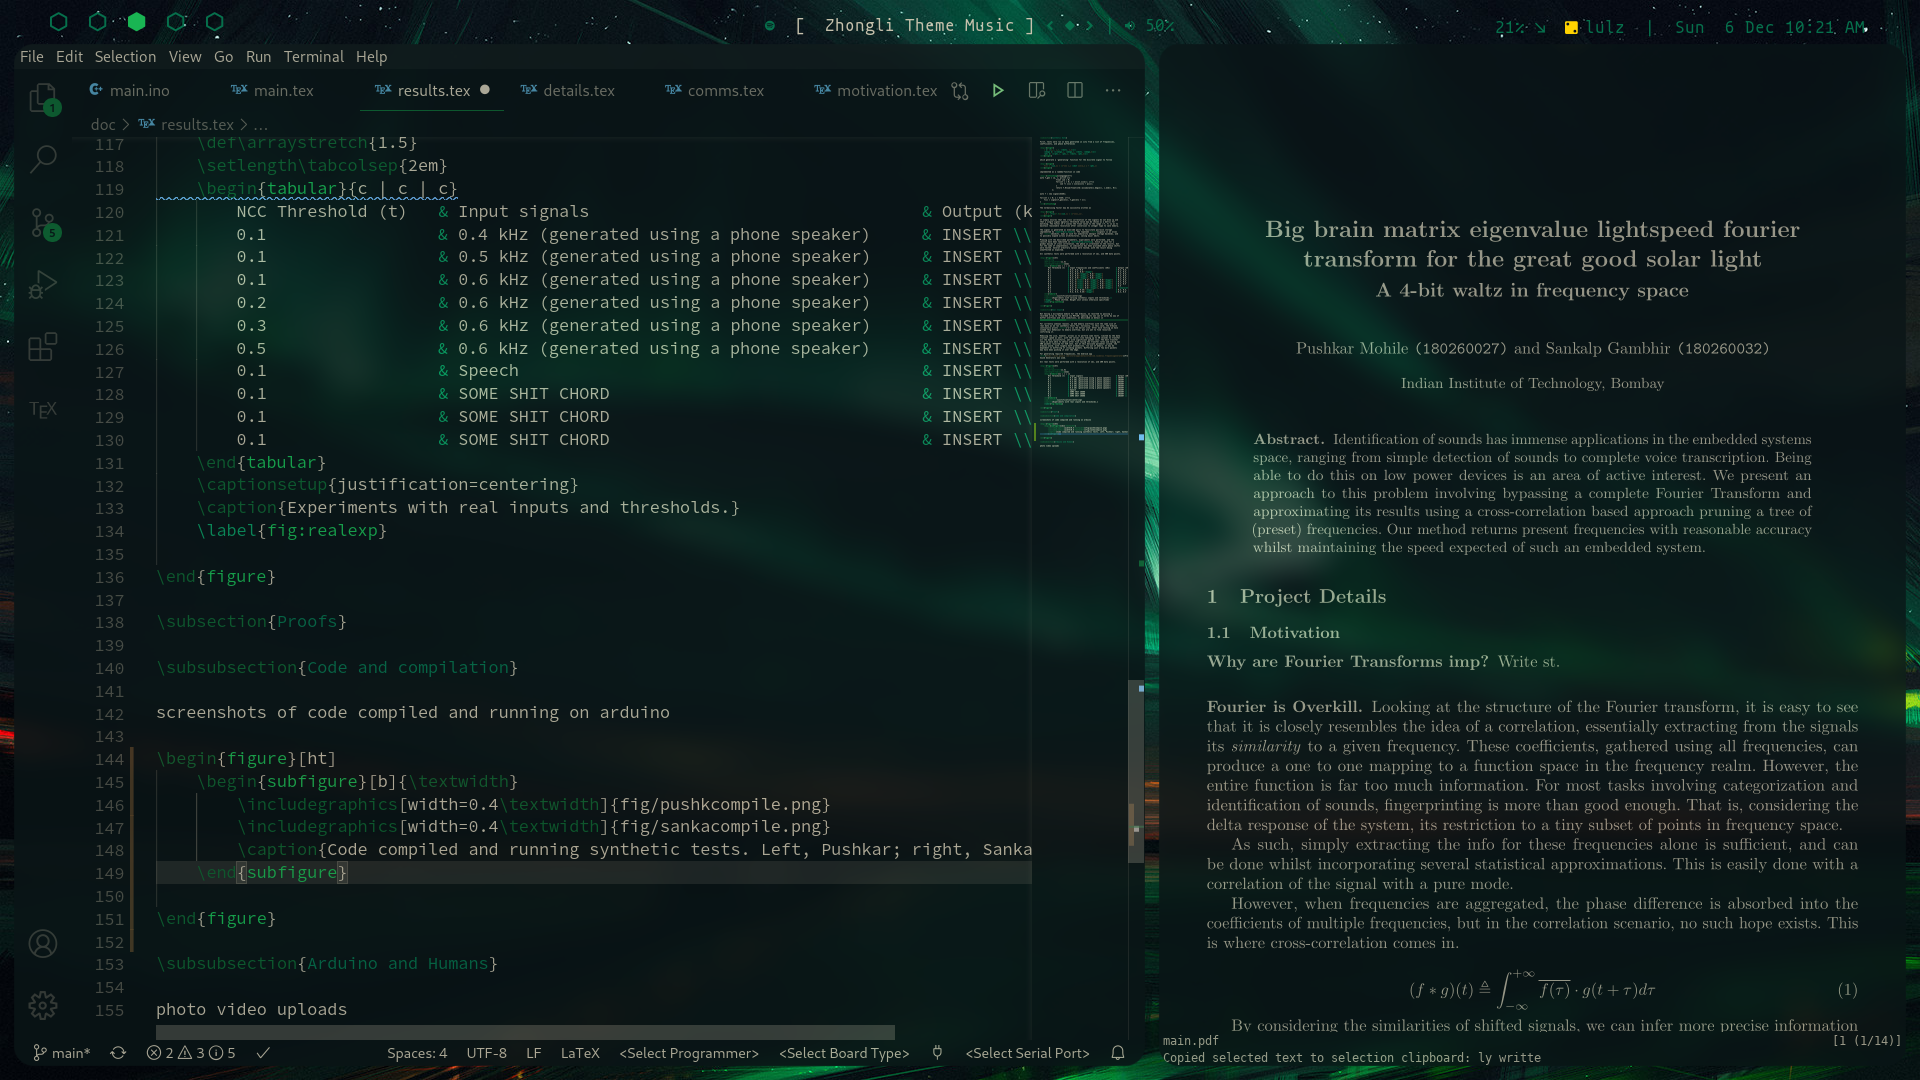
\includegraphics[width=0.7\textwidth]{fig/pushkcompile.png}
    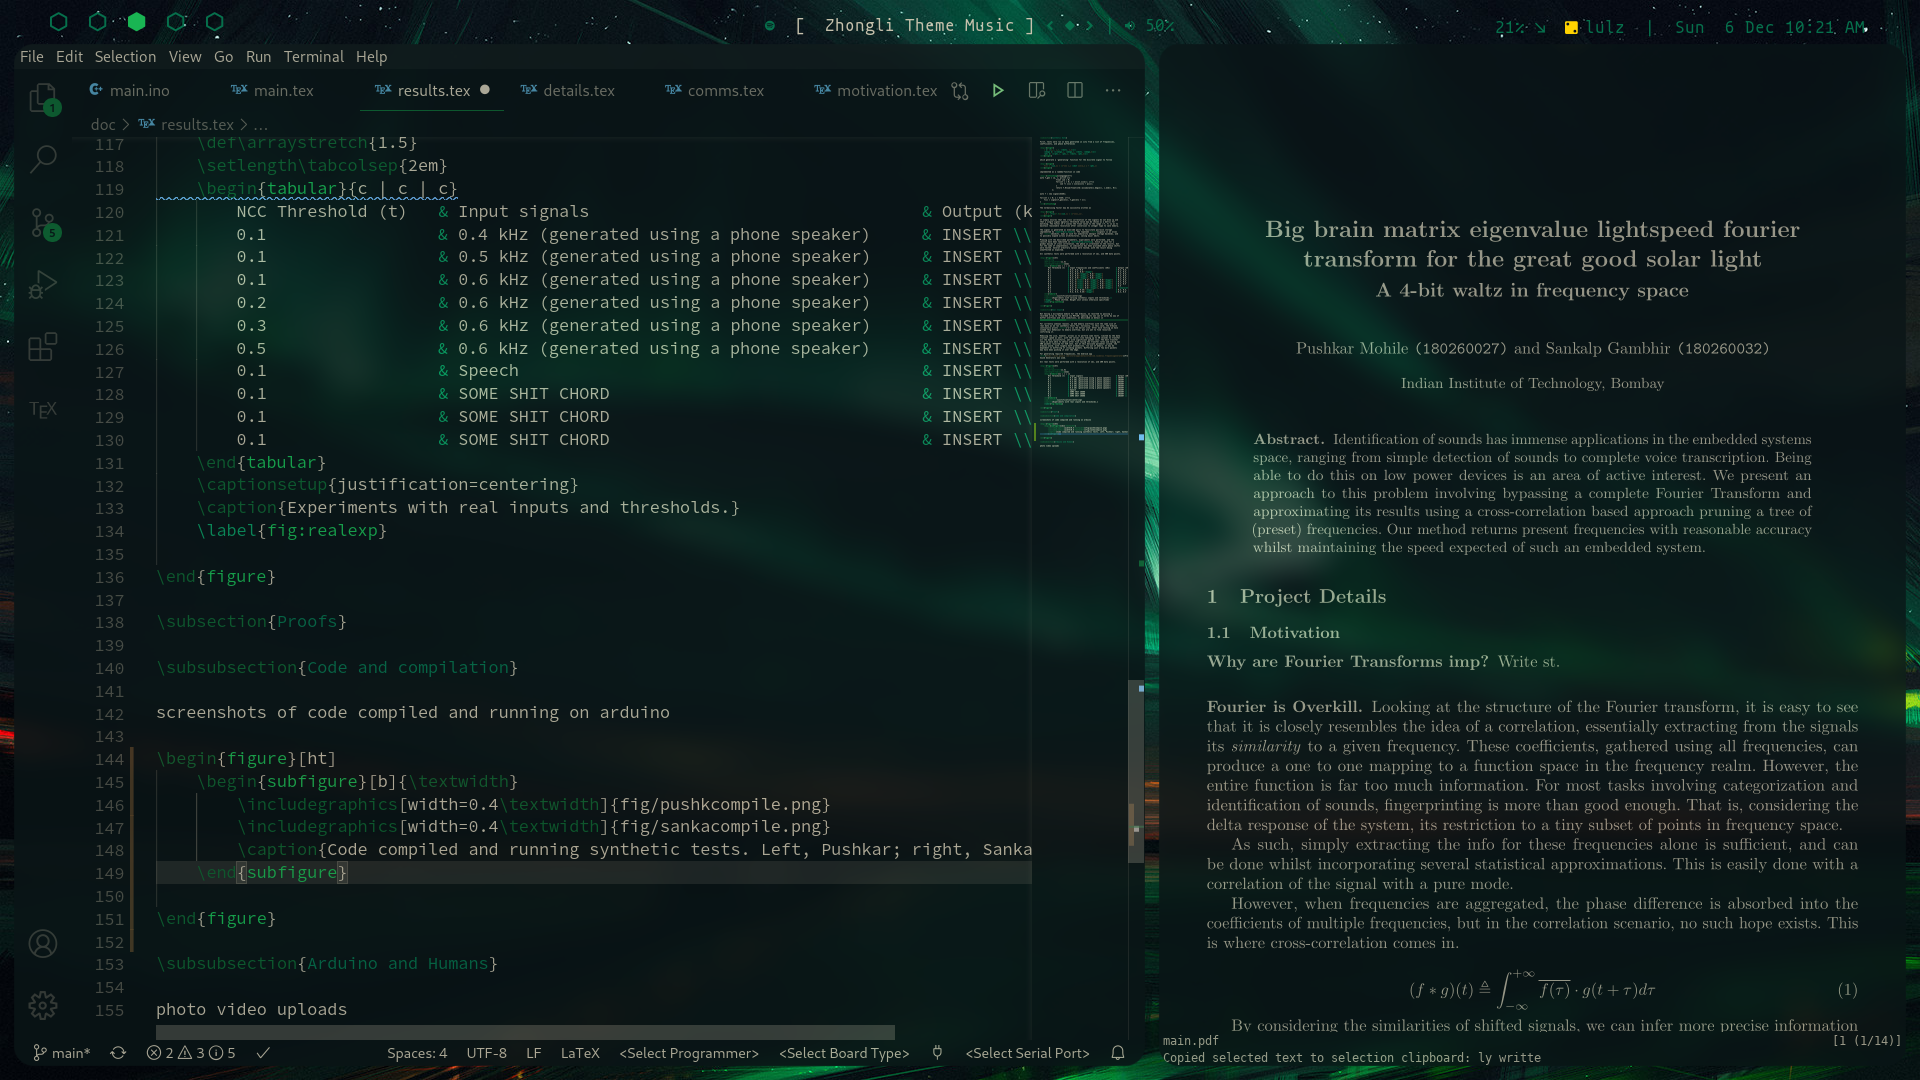
\includegraphics[width=0.7\textwidth]{fig/sankacompile.png}
    \caption{Code compiled and running synthetic tests. Left, Pushkar; right, Sankalp.}
\end{figure}

\begin{figure}[ht]
    \centering
    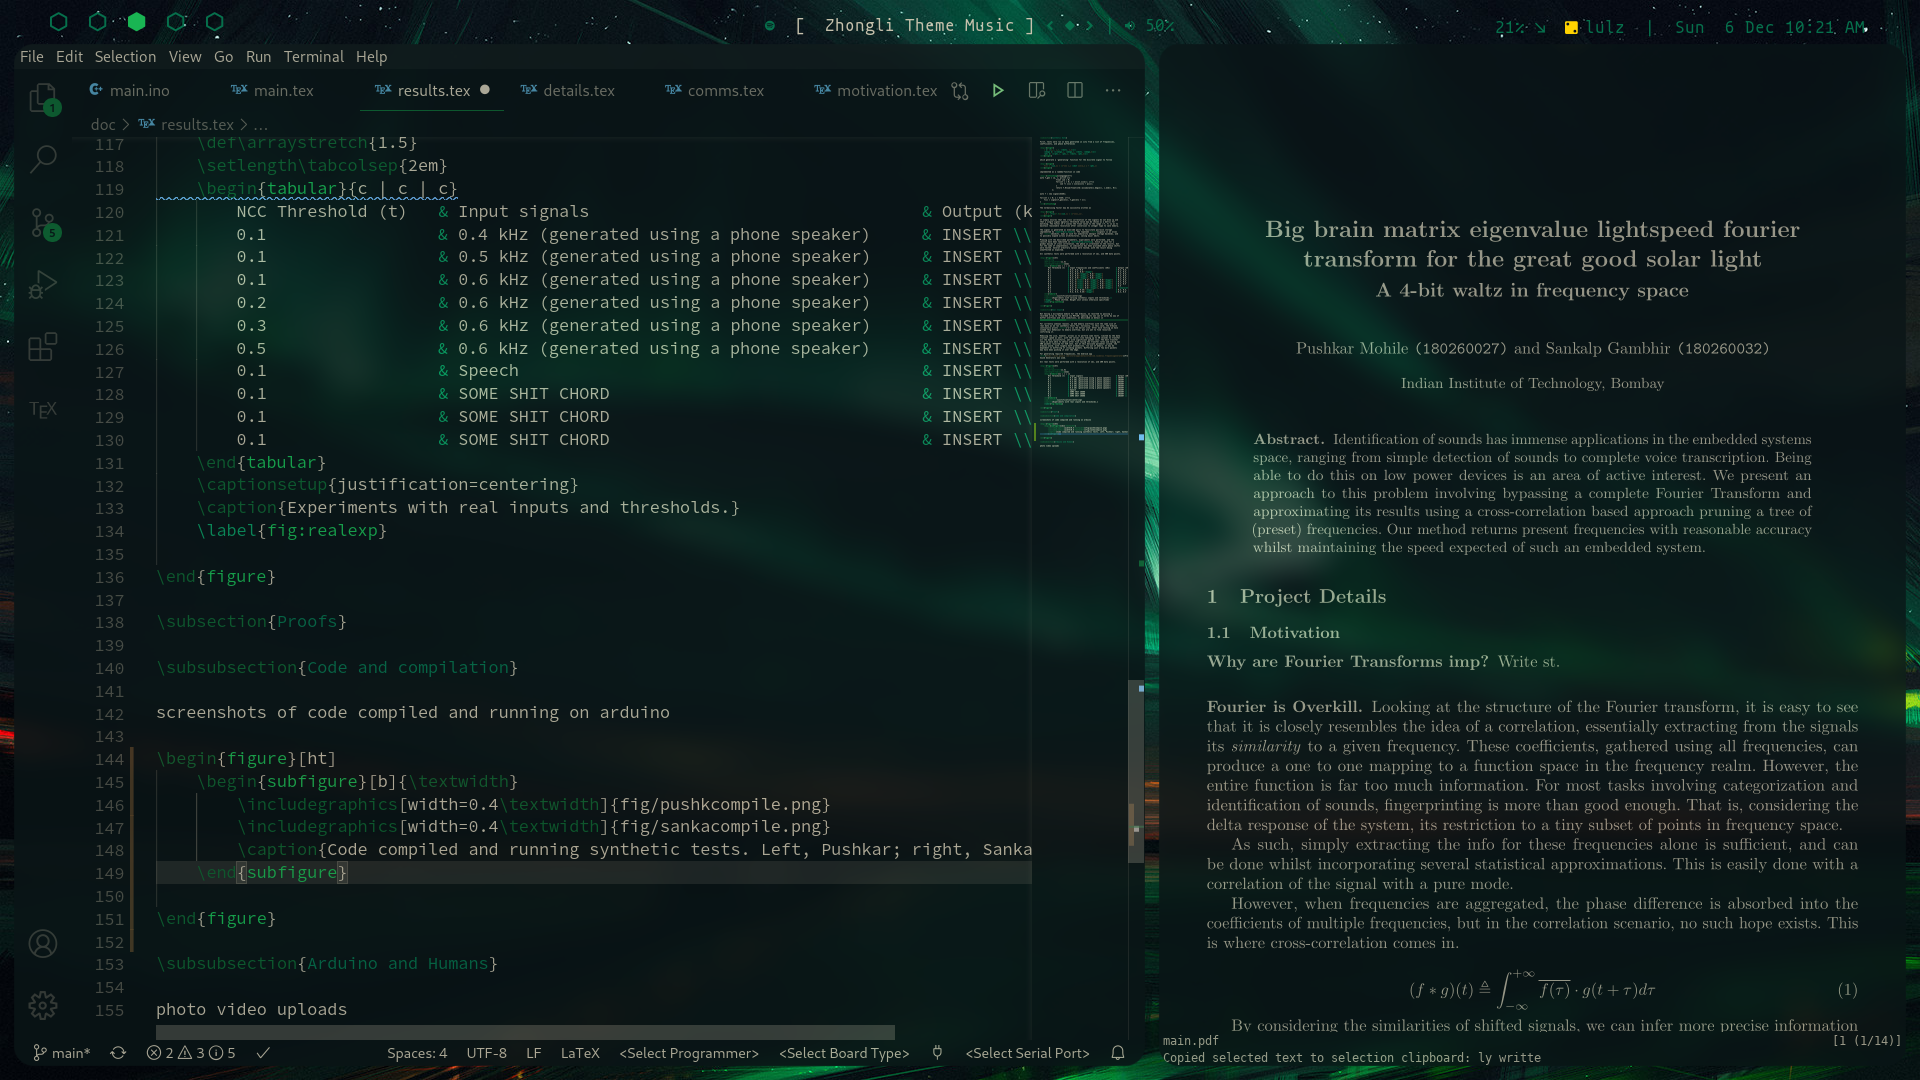
\includegraphics[width=0.7\textwidth]{fig/pushkreal.png}
    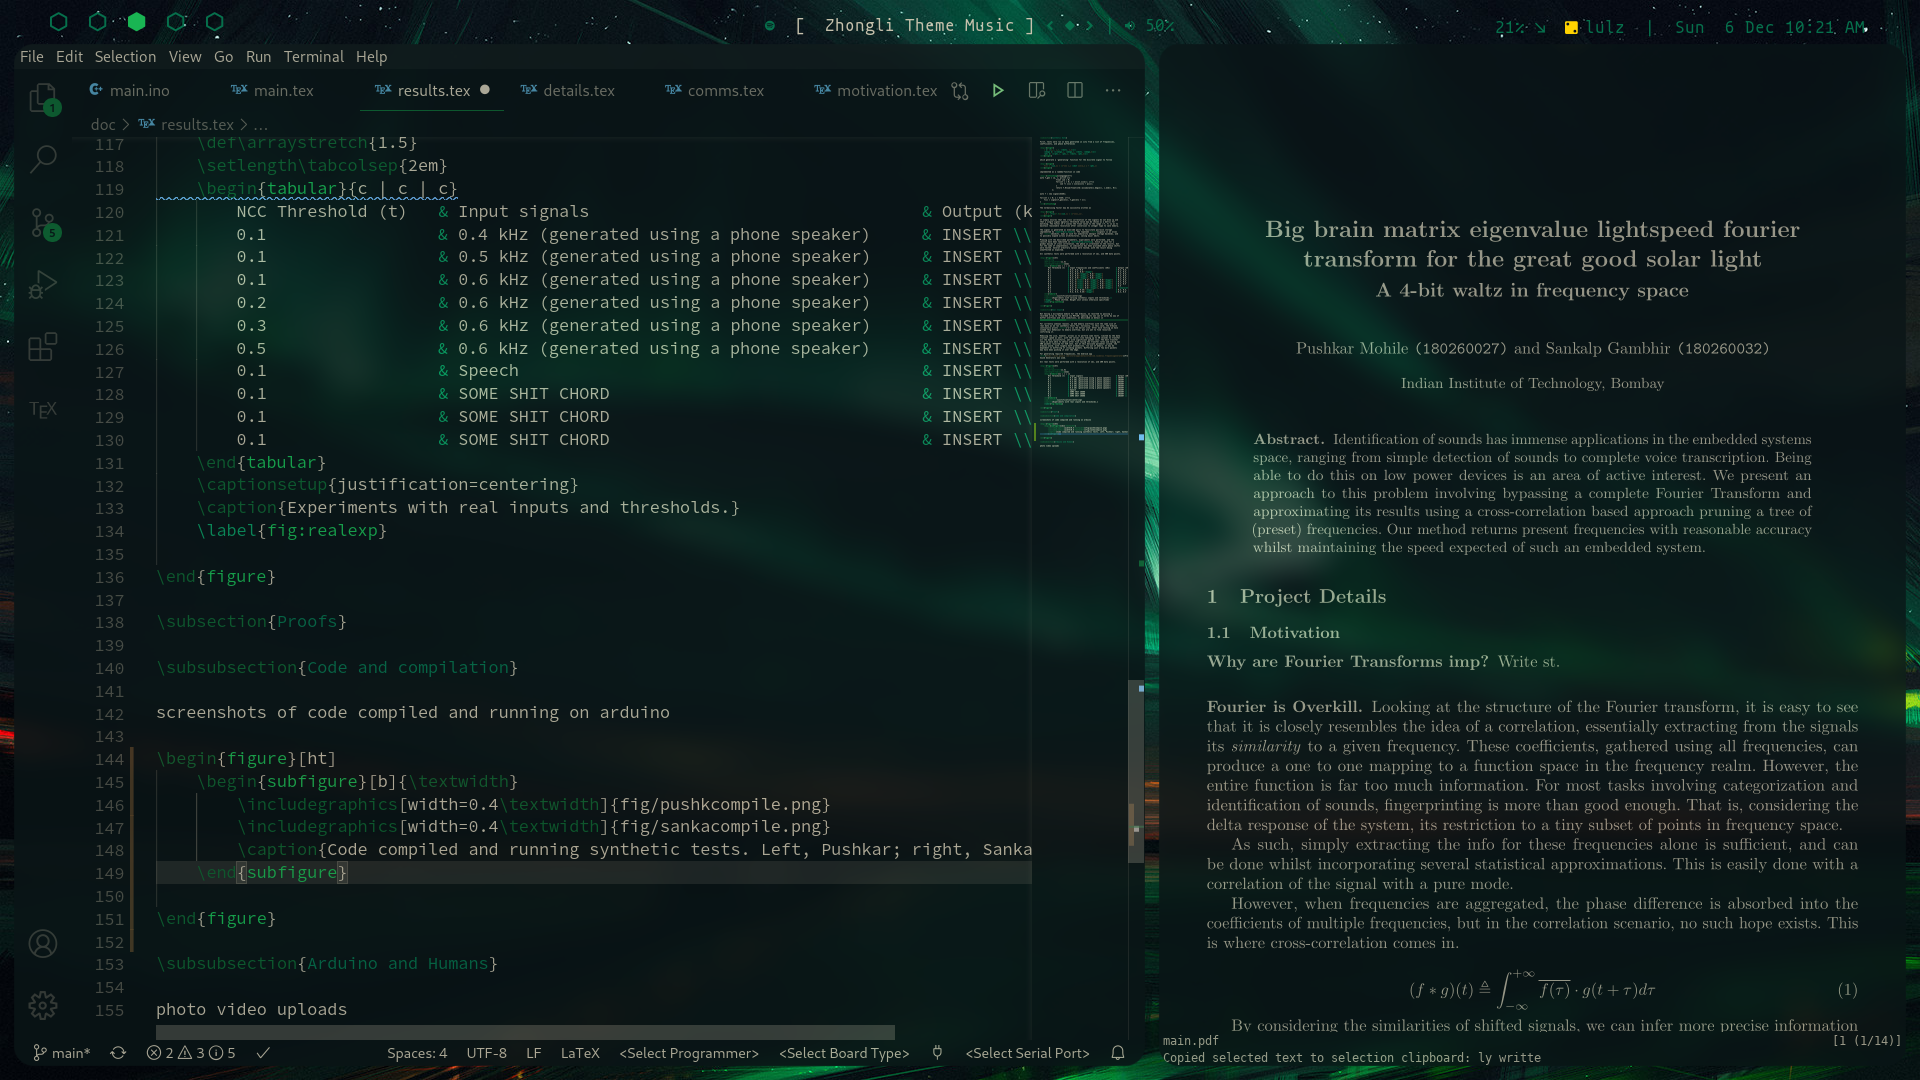
\includegraphics[width=0.7\textwidth]{fig/sankareal.png}
    \caption{Code running. Left, Pushkar; right, Sankalp.}
\end{figure}

\subsubsection{Arduino and Humans}

photo video uploads